% Created 2019-02-23 Sat 18:45
% Intended LaTeX compiler: pdflatex
\documentclass[11pt]{article}
\usepackage[utf8]{inputenc}
\usepackage[T1]{fontenc}
\usepackage{graphicx}
\usepackage{grffile}
\usepackage{longtable}
\usepackage{wrapfig}
\usepackage{rotating}
\usepackage[normalem]{ulem}
\usepackage{amsmath}
\usepackage{textcomp}
\usepackage{amssymb}
\usepackage{capt-of}
\usepackage{hyperref}
\author{Andrew Chen}
\date{\today}
\title{}
\hypersetup{
 pdfauthor={Andrew Chen},
 pdftitle={},
 pdfkeywords={},
 pdfsubject={},
 pdfcreator={Emacs 27.0.50 (Org mode 9.1.14)}, 
 pdflang={English}}
\begin{document}

\tableofcontents

\section{Regression}
\label{sec:org9ebda85}

\subsection{Warmup}
\label{sec:org56f4fe9}

\begin{itemize}
\item An n x d matrix is one that has n rows and d columns
\item Vector Norms:
\begin{itemize}
\item l\(_{\text{p}}\) norm: ||x||\(_{\text{p}}\) = (\(\sum_{\text{i}}\) |x\(_{\text{i}}\)|\(^{\text{p}}\))\(^{\text{1/p}}\)
\item l\(_{\text{2}}\) norm (Euclidean Norm): ||x||\(_{\text{2}}\) = (\(\sum_{\text{i}}\) x\(_{\text{i}}^{\text{2}}\))\(^{\text{1/2}}\)
\item l\(_{\infty}\) norm: ||x||\(_{\infty}\) = \(\max_{\text{i}}\)|x\(_{\text{i}}\)|

\begin{figure}[htbp]
\centering
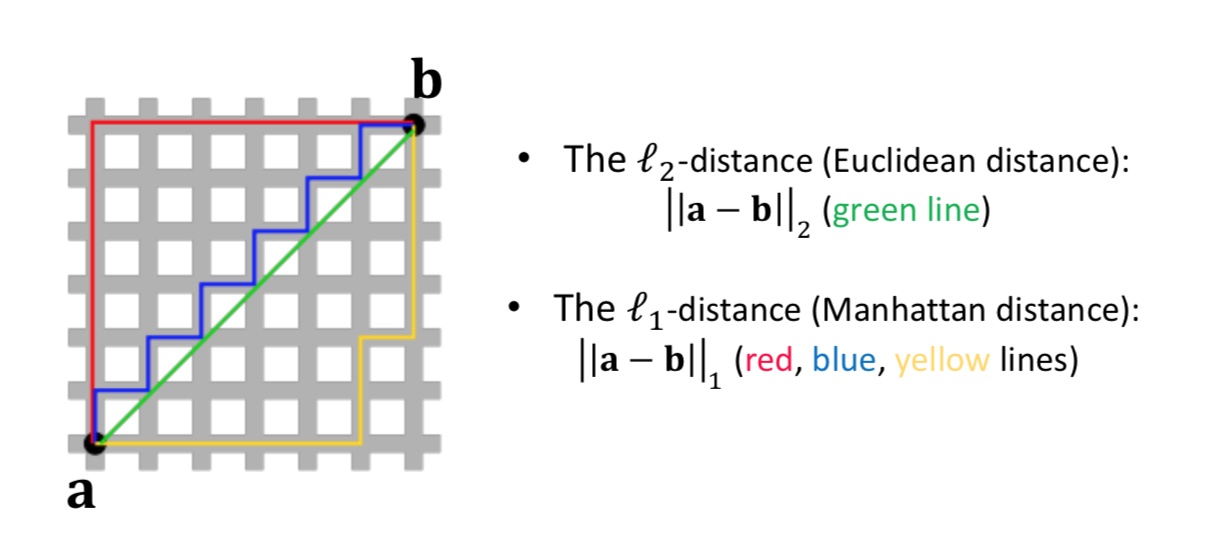
\includegraphics[width=.9\linewidth]{./images/norm_distances.png}
\caption{Norm distances}
\end{figure}
\end{itemize}
\end{itemize}

\subsection{Rank}
\label{sec:org3e75e31}

\begin{itemize}
\item Rank: The number of linearly independent rows (or columns).
\item Full Rank: a square matrix is full rank if the rank equals to \#columns.
\end{itemize}

\subsection{Eigenvalue Decomposition}
\label{sec:org48114b0}

\begin{itemize}
\item let 𝐀 be any 𝑛×𝑛 symmetric matrix.
\item Eigenvalue decomposition: A = \(\sum^{\text{n}}_{\text{i=1}}\) \(\lambda_{\text{i}}\)v\(_{\text{i}}\)v\(^{\text{T}}_{\text{i}}\)
\item Eigenvalues satisfy |\(\lambda_{\text{1}}\)| \(\ge\) |\(\lambda_{\text{2}}\)| \(\ge\) \dots{} \(\ge\) |\(\lambda_{\text{n}}\)|
\item Eigenvectors satisfy v\(^{\text{T}}_{\text{i}}\)v\(_{\text{j}}\) = 0 for all i \(\ne\) j
\item \textbf{\textbf{A}} is a full rank iff all the eigenvalues are nonzero
\end{itemize}

\subsection{Least Squares Regression with Gradient Descent}
\label{sec:org57bb7fa}

\begin{enumerate}
\item Least squares regression model: x\{\hat{x}\}
\end{enumerate}
\end{document}
